During the duration of the dedicated photon run all SVT hybrids and APV25 
readout chips were configured to their nominal operating 
points~\cite{Jones:1069892} while all sensors were reverse-bias at 180~V.  The 
sensors were operated within a temperature range of  20 to 24$^\circ$C 
throughout the test run. Multiple calibration runs established a noise level of 60-68 
ADC counts ($\approx$ 750 - 850 electrons)  which was stable across all hybrids. With a linear gain up to $\approx 3$~MIPs, the 
cluster charge for hits on a track follow the characteristic Landau shape (see Fig.~\ref{fig:cluster_pulse}) with a 
mean of about 25,500~e$^{-}$ as expected. 
%This signal response gives a signal-to-noise ratio of about 25.5. 
\begin{figure}[h]
    % TODO: The pulse plot needs to be remade such that the x-axis is time 
	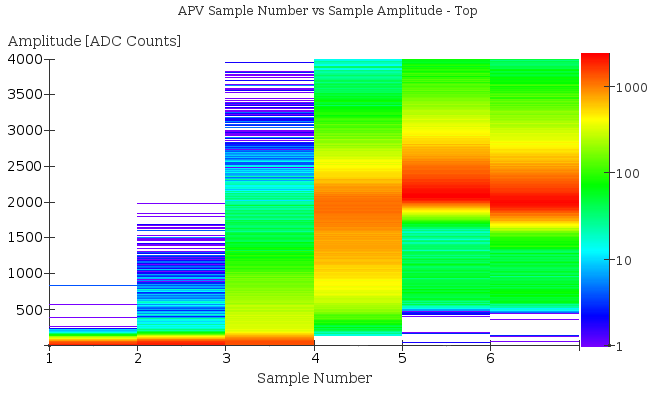
\includegraphics[width=0.49\textwidth]{test2012/svtperformance/svt_calib/08062012_run1351_samples_vs_amplitude.png}
	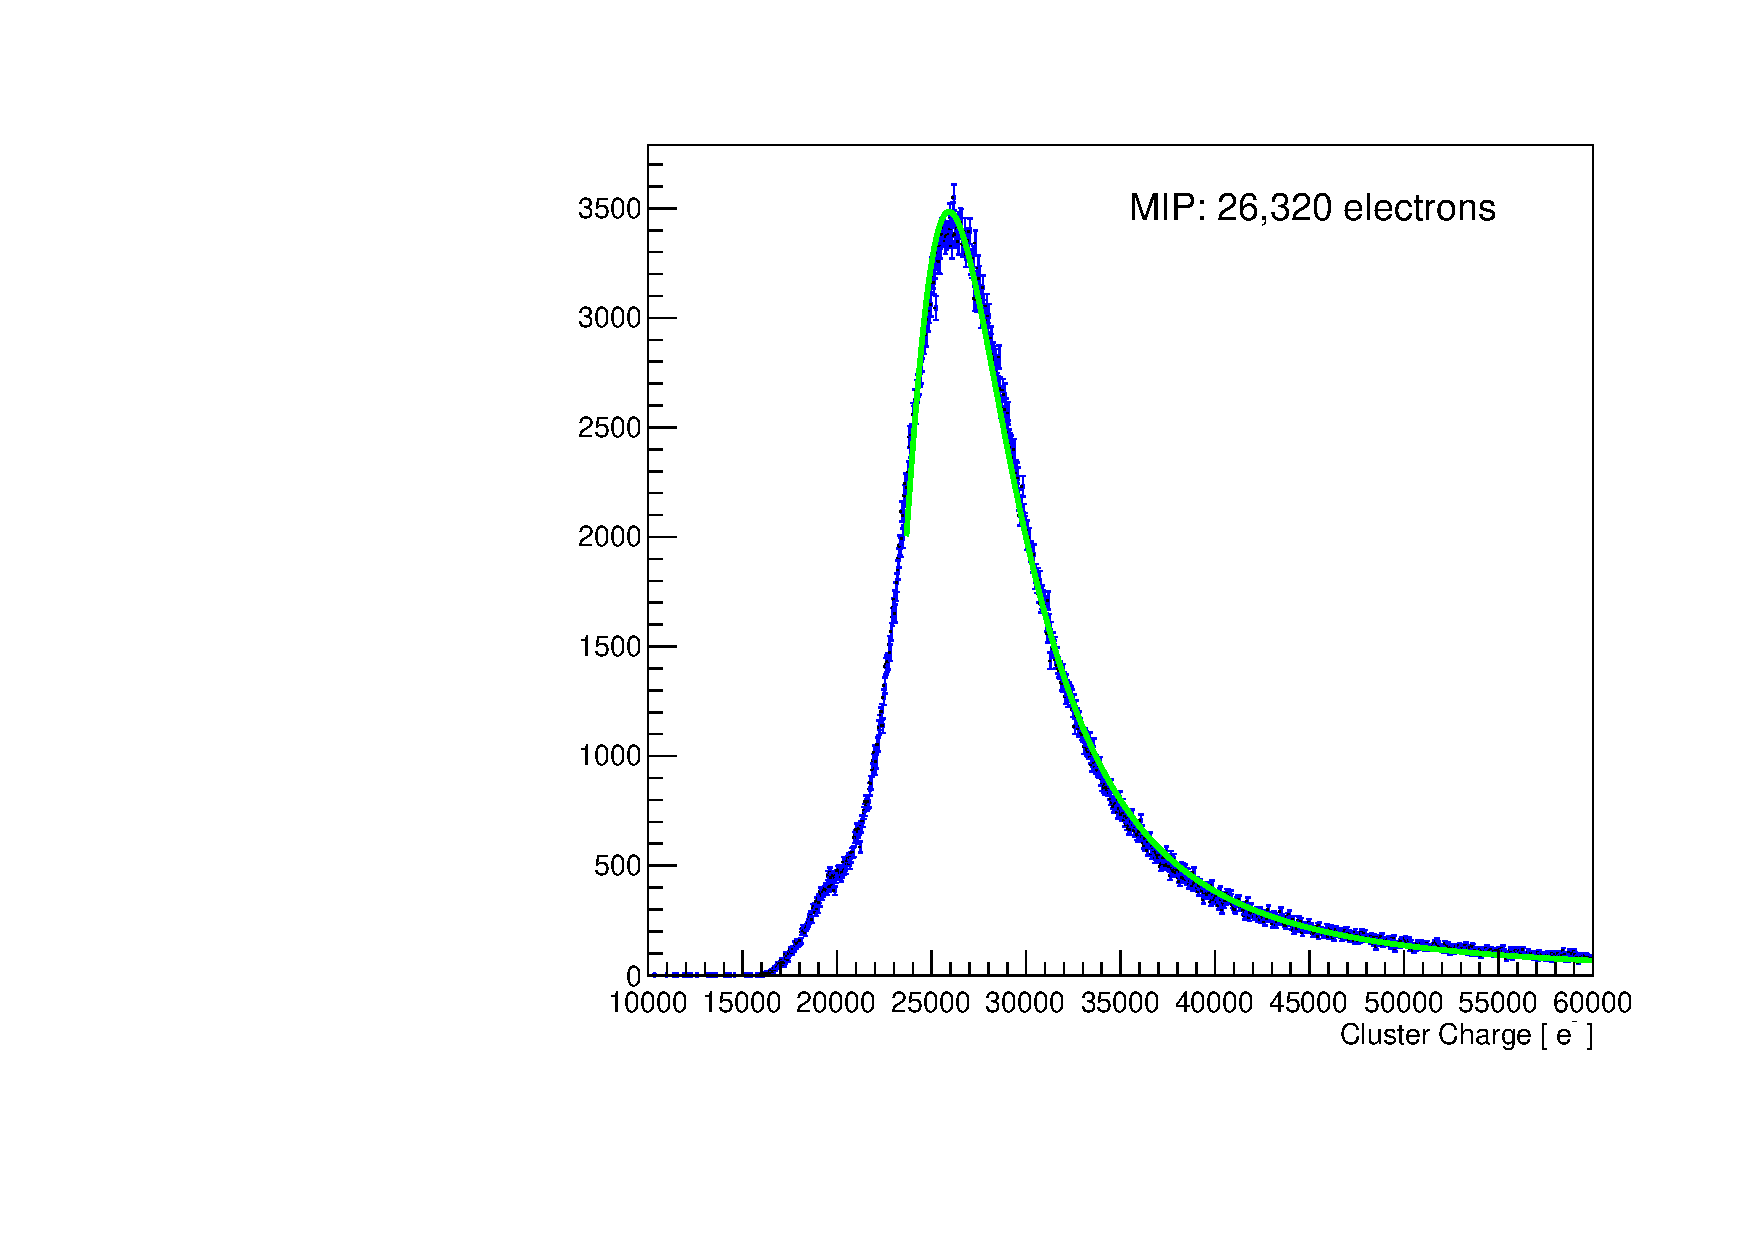
\includegraphics[width=0.49\textwidth]{test2012/svtperformance/svt_calib/run1351_mip_small.pdf}
    \caption{The six pedestal subtracted samples associated with a hit on a track 
             are shown on the left plot along with a distribution of the cluster
             charge exhibiting the characteristic Landau shape on the right. 
            }
	\label{fig:cluster_pulse}
\end{figure}


One of the important tests of the SVT was the operation of the APV25 chips in multi-peak readout mode 
discussed in Sec.~\ref{sec:svt}. The six samples of the APV25 pulse shaper output 
are fitted to an ideal $CR-RC$ function to extract the amplitude and the $t0$ of the hit. 
The typical cluster shape obtained is shown in Fig.~\ref{fig:cluster_pulse} also demonstrates that the SVT was well timed in to the trigger with the rise of the pulse at the 3rd sampling point.
After clustering hits on a sensor, the hit time for each cluster is computed as the amplitude-weighted average of 
the fitted $t0$ channel times. The $t0$-resolution is studied by comparing the cluster hit time with the average of all cluster hit times, the "track time". Figure~\ref{fig:tracktime} shows the track time, with the expected jitter due to clock phase and trigger, and the residual to the individual cluster times. 
\begin{figure}[h]
%	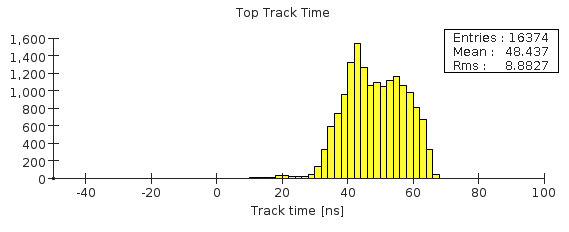
\includegraphics[width=0.7\textwidth]{test2012/svtperformance/track_time_top}
%	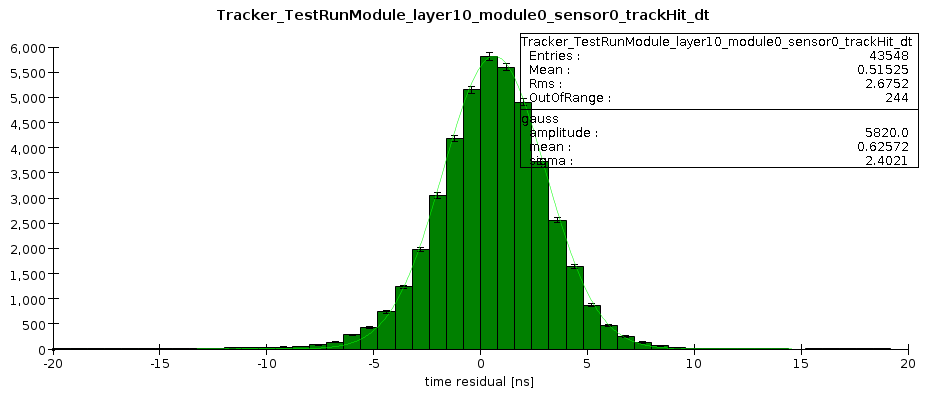
\includegraphics[width=0.7\textwidth]{test2012/svtperformance/timeres}
	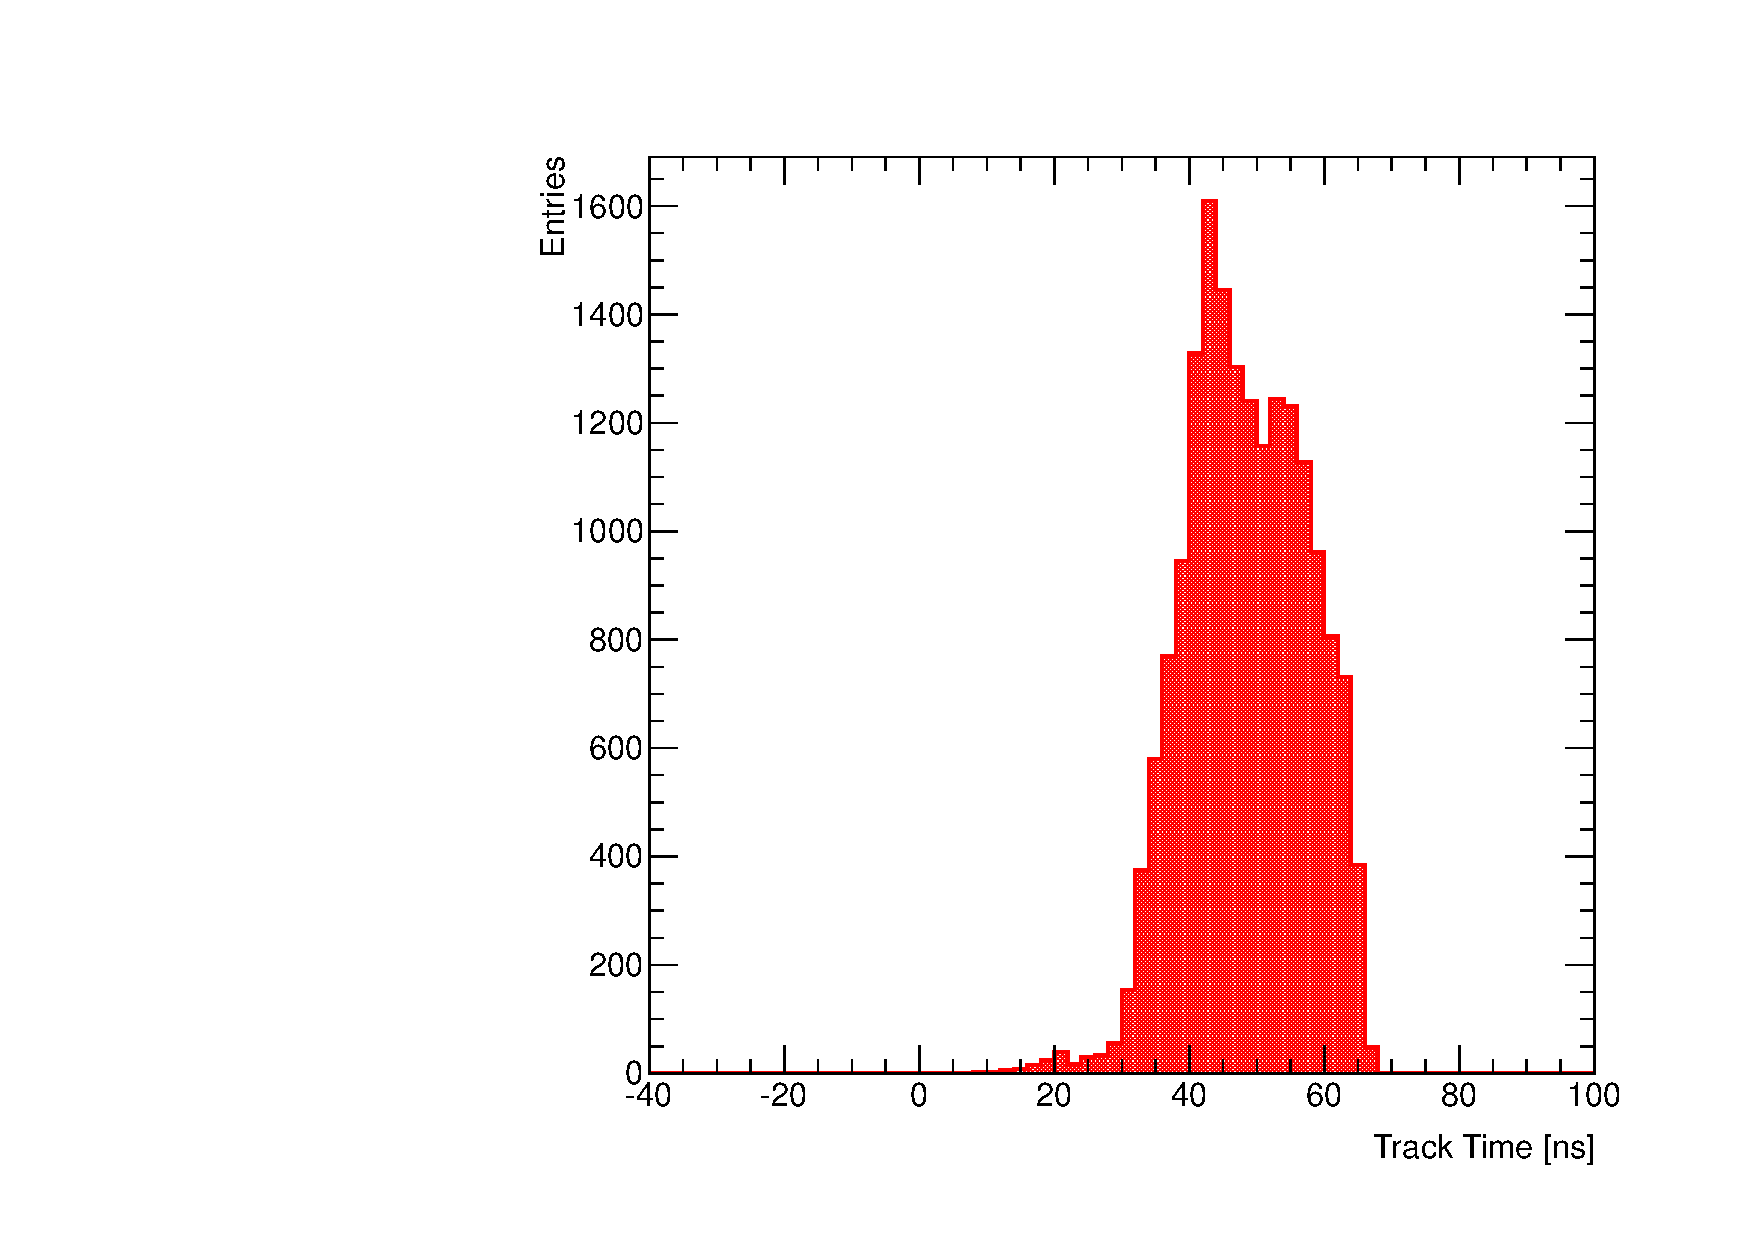
\includegraphics[width=0.49\textwidth]{test2012/svtperformance/top_track_time.pdf}
	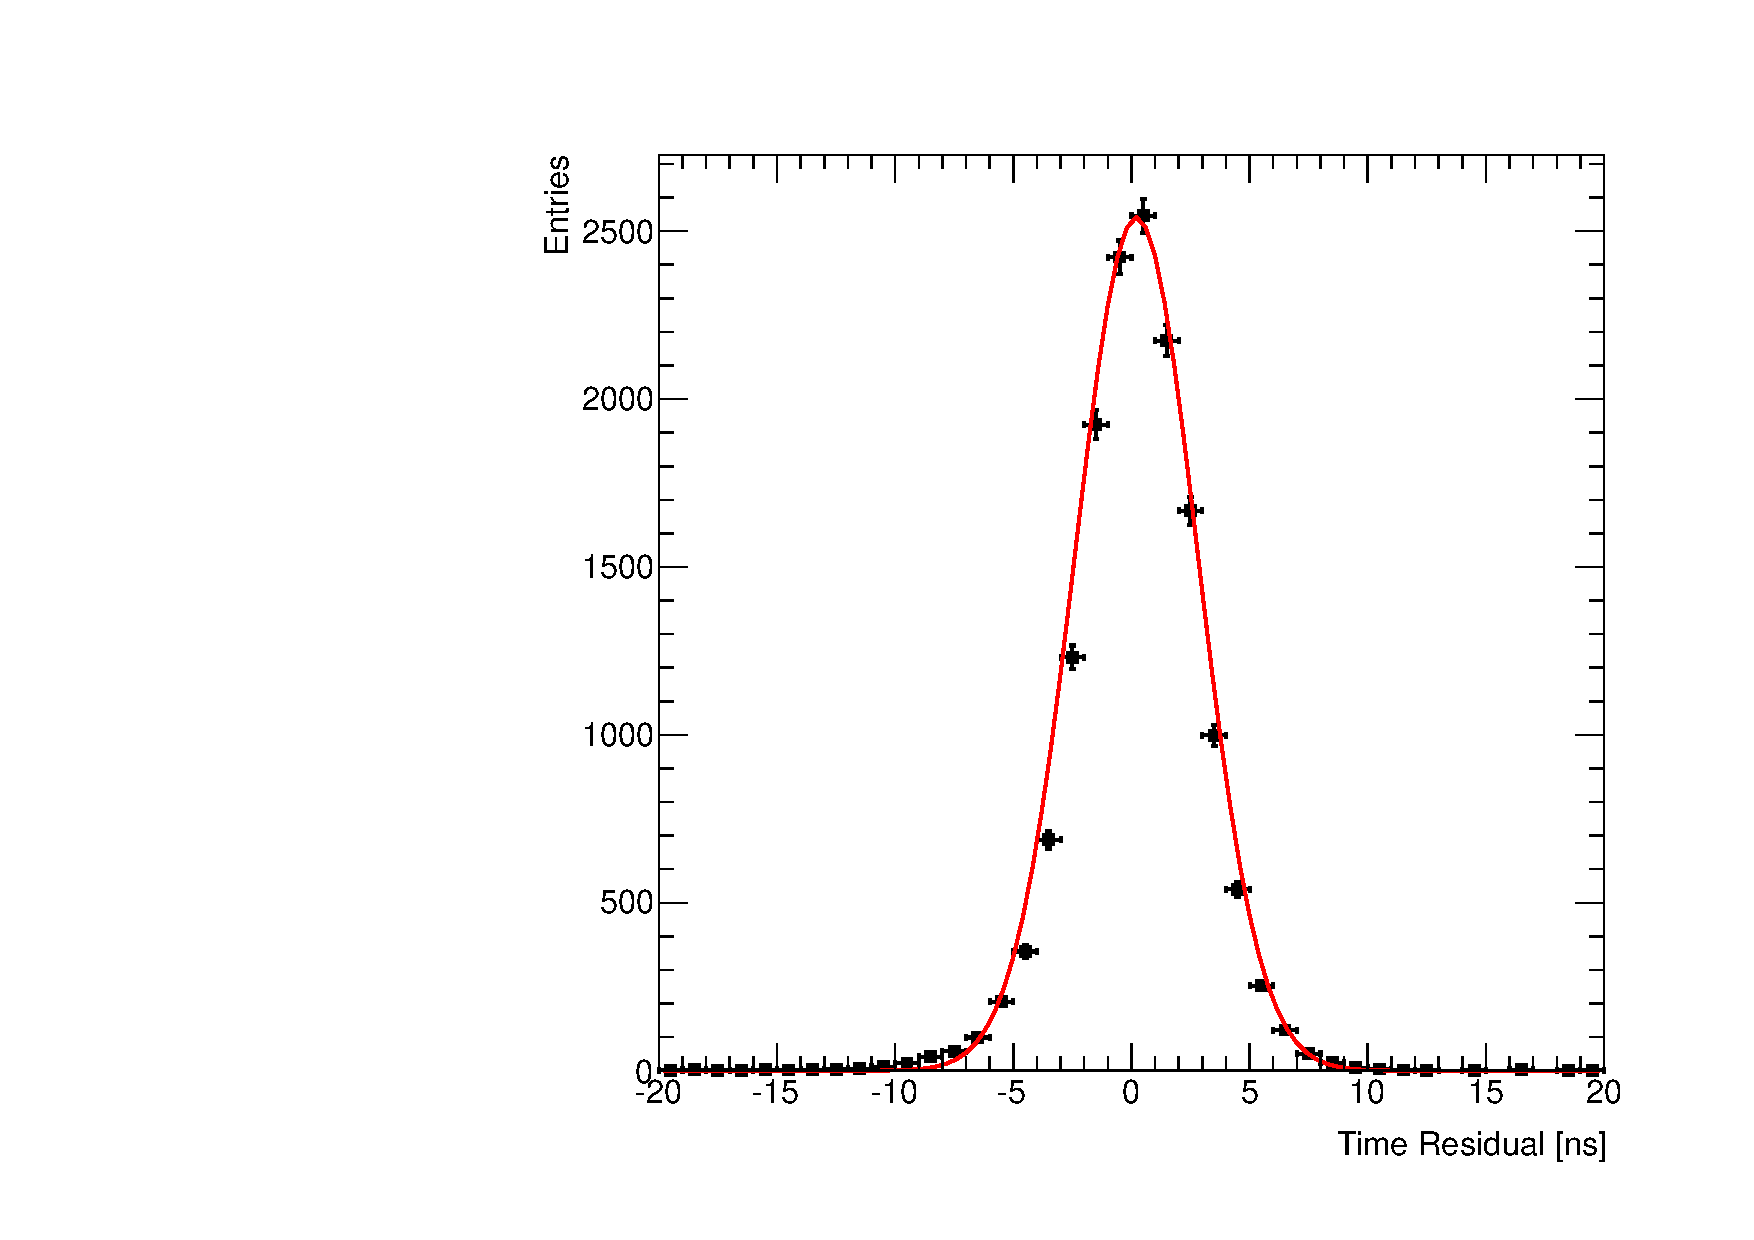
\includegraphics[width=0.49\textwidth]{test2012/svtperformance/t0_resolution.pdf}
	\caption{\small{Track time distribution (left) and cluster time residual (right). The 
	track time is measured relative to the APV25 clock. The width of the distribution is due to 
	trigger jitter (24~ns jitter in the tracker readout clock, plus 16~ns jitter in the trigger system). 
	The cluster time residual is for a representative sensor relative to the track time.}}
	\label{fig:tracktime}
\end{figure}
After correcting for offsets from each sensor (time-of-flight, clock phase) the extracted $t0$ resolution is 2.6~ns (larger than the 2.4~ns due to correlations between the cluster and "track" times). This is somewhat worse than the $\approx 2$ ns resolution expected in Sec.~\ref{sec:performance} which we attribute to our pulse shape fit procedure function (see Appendix for more details). 

Throughout the duration of the test run, approximately 97\% of the 12,780 SVT 
channels were found to be functional.
The identified dead or noisy channels were largely attributed to a 
known noisy sensor and a few noisy or misconfigured chips which will be resolved for future running. The 
increased noise resulted in occupancies and data rates that were higher than what were expected from simulation.
However, after masking out all known noisy channels found during the commissioning of the SVT, good agreement 
between simulation and test run data was achieved as shown on Fig.~\ref{fig:data_rates_data_mc_cmp}.
\begin{figure}[h]
    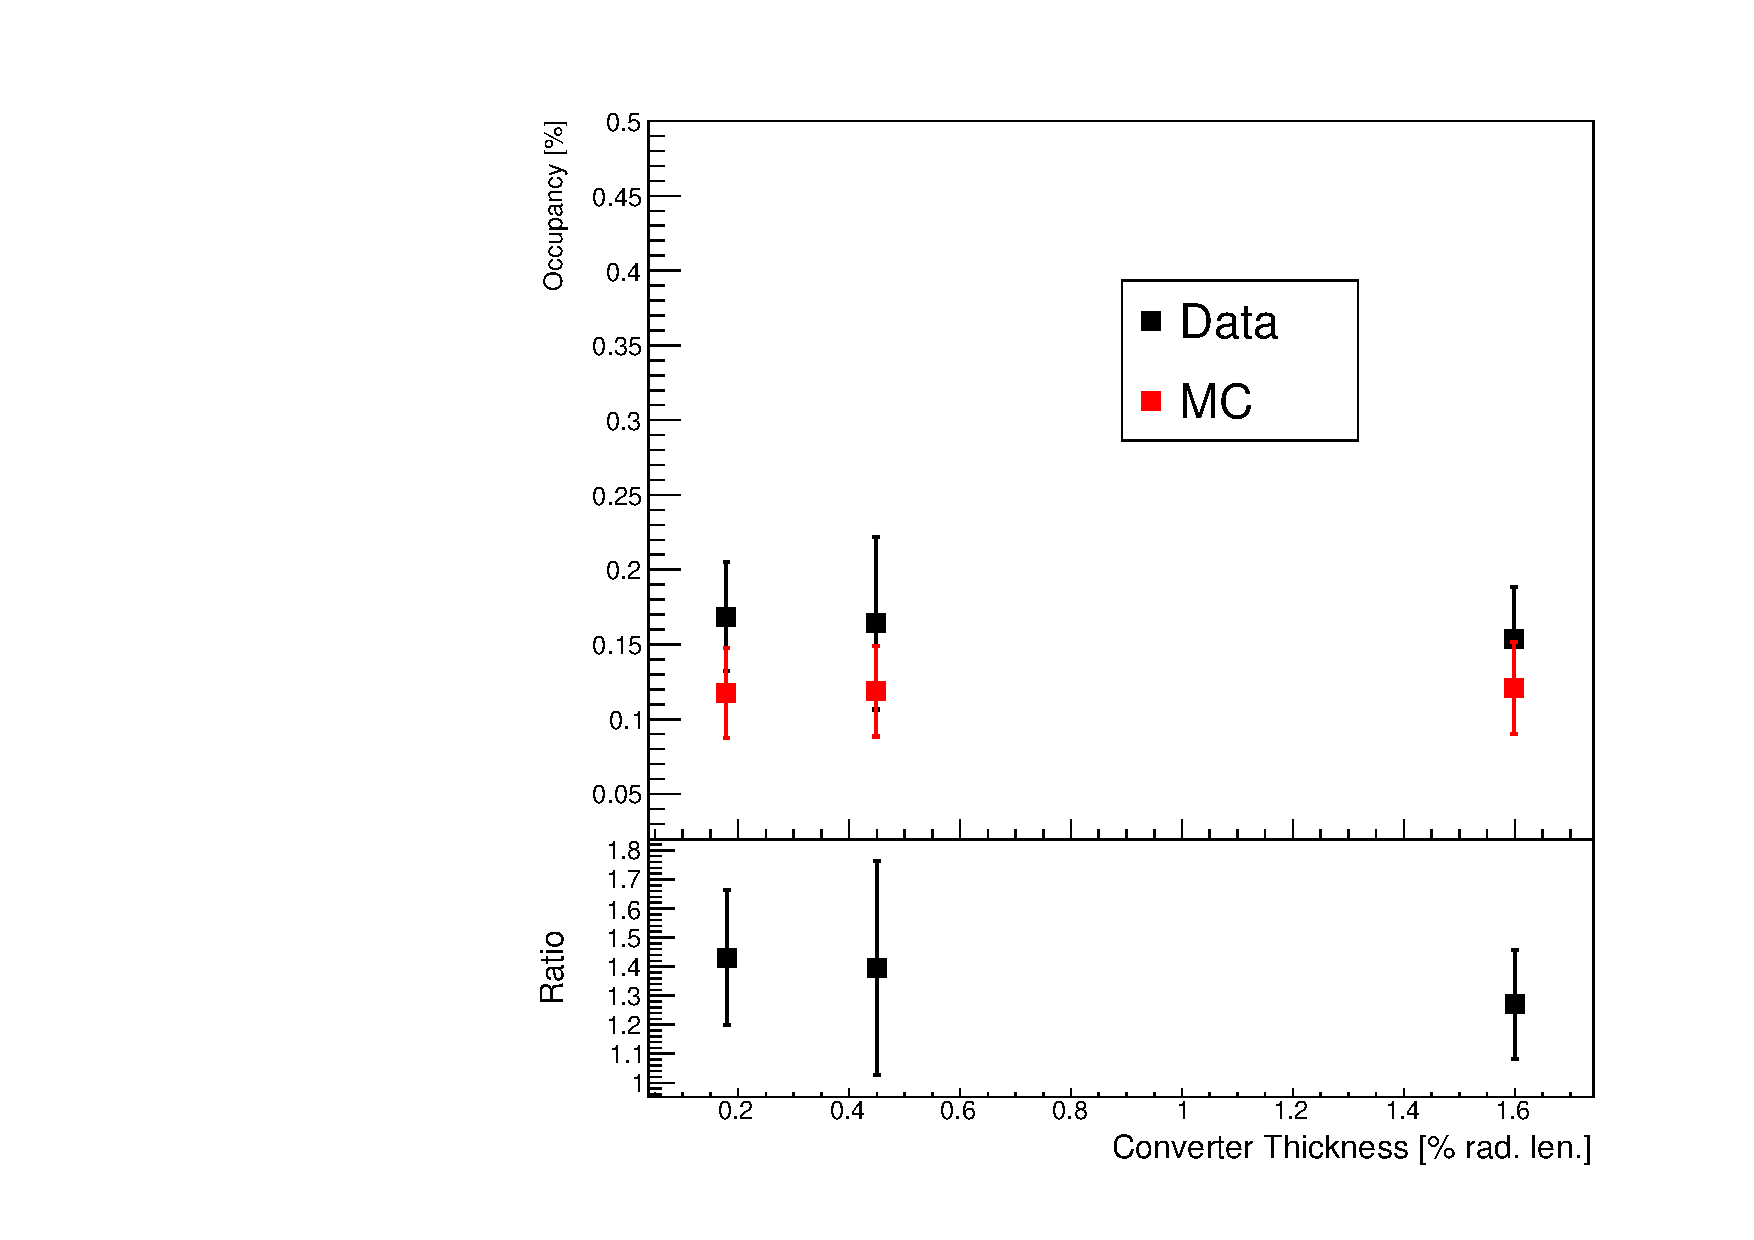
\includegraphics[width=0.49\textwidth]{test2012/svtperformance/daq/occupancy_vs_target_thick.pdf}
    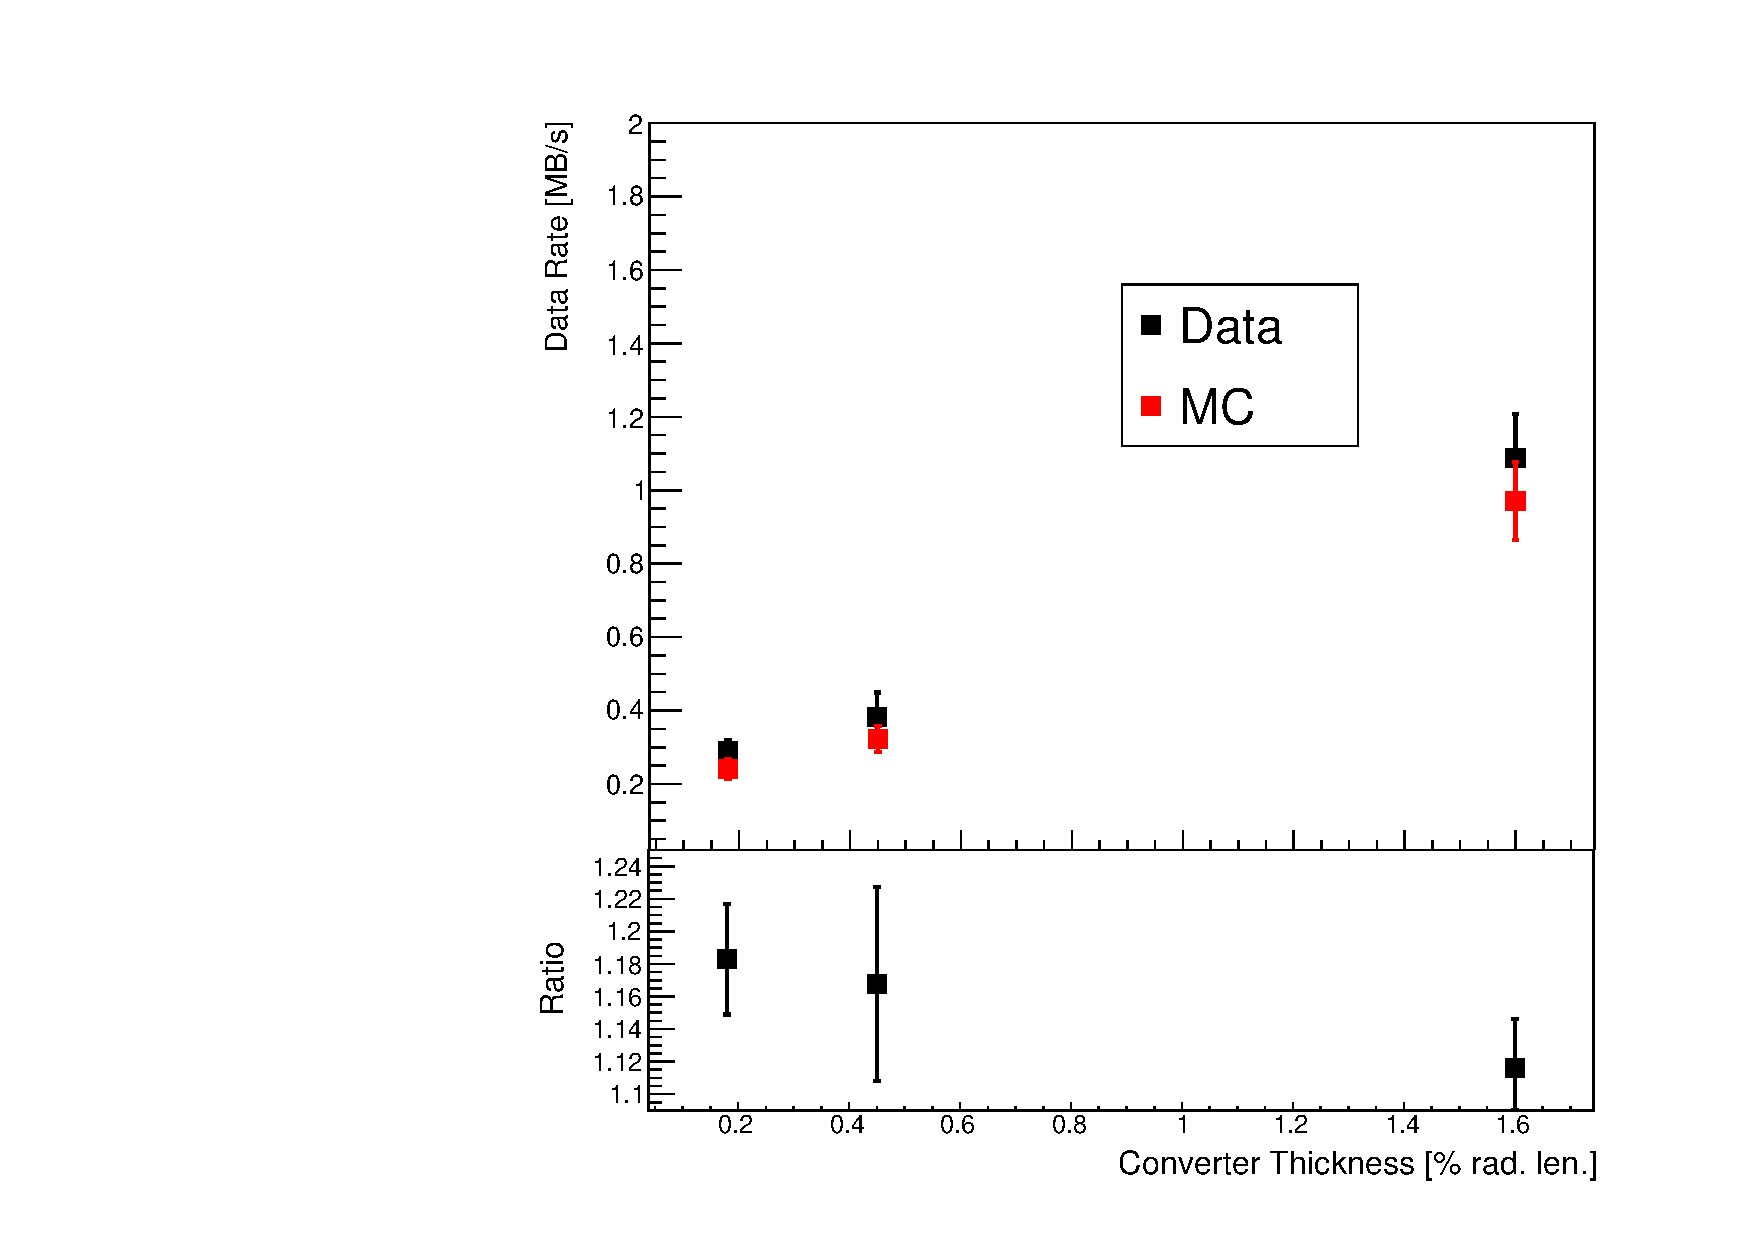
\includegraphics[width=0.49\textwidth]{test2012/svtperformance/daq/data_rate_vs_target_thick.pdf}
        \caption{ { \small
                    Comparison of SVT occupancy and data rates between test run data and that expected from simulation after noisy channels are masked.
                } }
	\label{fig:data_rates_data_mc_cmp}
\end{figure}
Similarly, the hit efficiency was measured to be above 98\% for known good layers, see Fig.~\ref{fig:hit_efficiency}.
\begin{figure}[h]
    	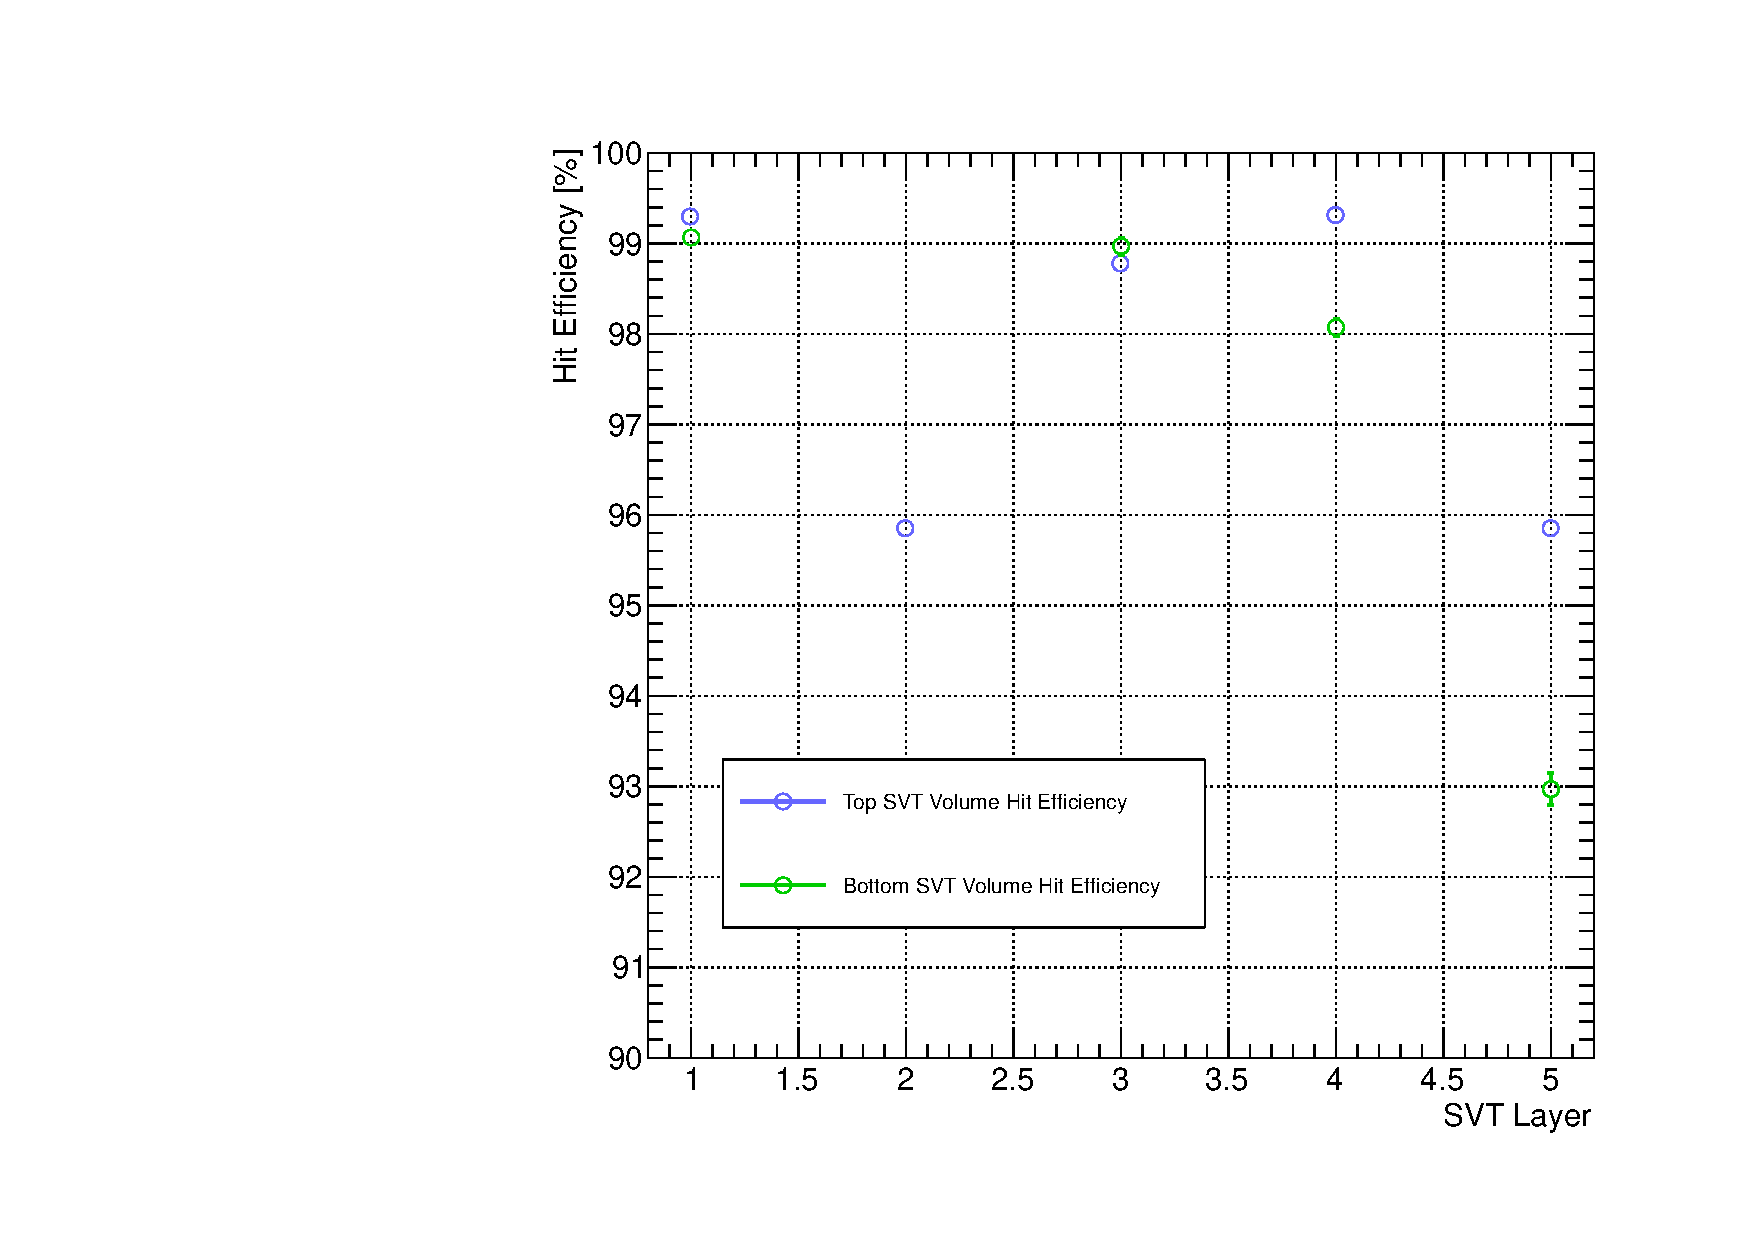
\includegraphics[width=.95\textwidth]{test2012/svtperformance/trk_performance/hit_efficiency_vs_layer.pdf}
%    	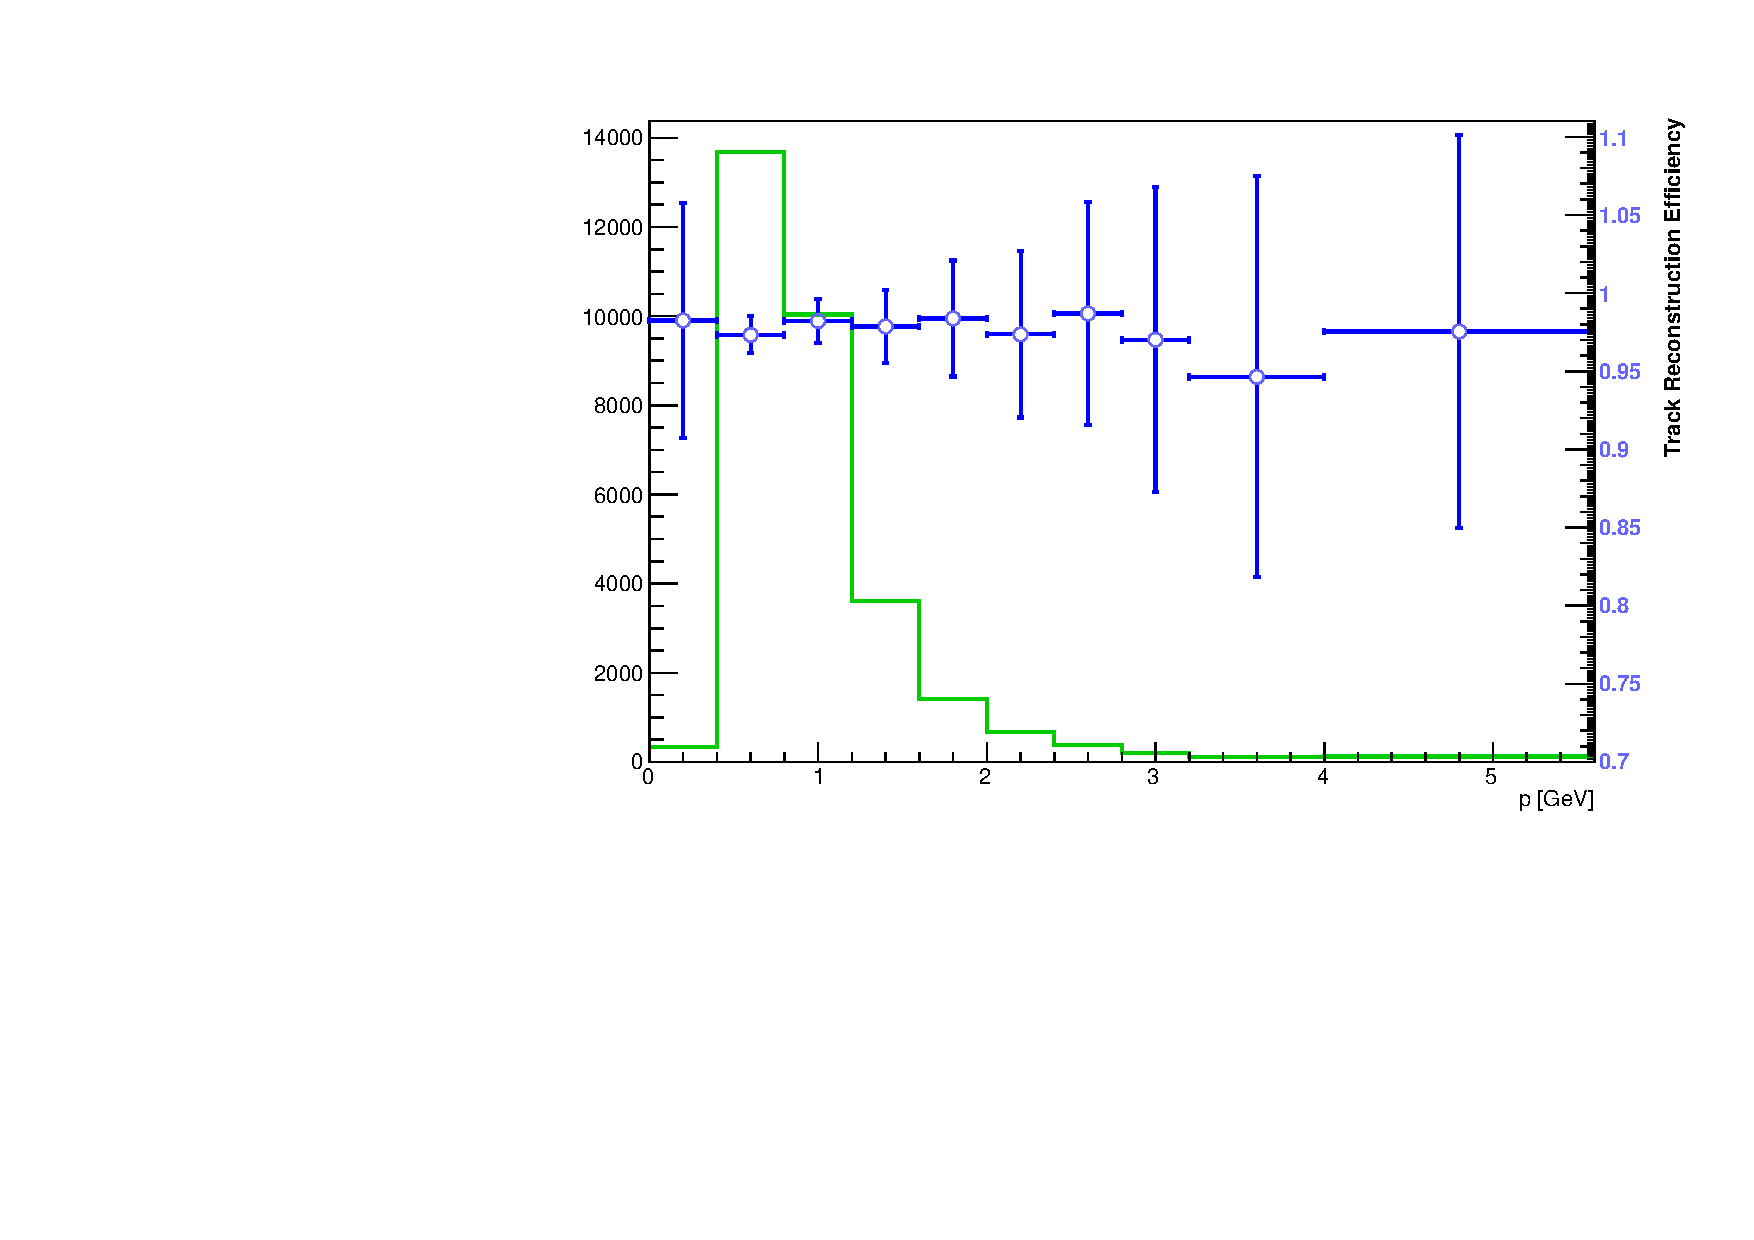
\includegraphics[width=0.49\textwidth]{test2012/svtperformance/trk_performance/track_reco_efficiency.pdf}
        \caption{{\small The hit reconstruction efficiency as a function of detector layer. The variation across the layers can be explained by known DAQ issues.}} 
	\label{fig:hit_efficiency}
\end{figure}
Further details can be found in the Appendix. 
